\subsubsection{Group Permissions}

\paragraph{Extending Individual Access Control}

Group permissions extend the above system for individual permissions and require the use of smart contracts.

Whilst our application is intended to be fully decentralised, the key stakeholders for some applications (such as health care) may require access to the network to administrate. One example of this is the involvement of the GMC in validating doctor identities. If a doctor has not been registered, or has been struck off, they should not have any access to patient data (even if they claim to be a doctor). They should only have access should the GMC validate that they are in fact a valid doctor.

The idea of a group administrator, such as the GMC, conflicts with the idea of the data owner maintaining full access control and administration. However, should the data owner decide that the group should no longer have any access or wishes to change group permissions, they are able to do so.

To facilitate this, let's take a look at the architecture of a group's interactions with a particular identity's contract.

\begin{figure}[H]
  \centering
  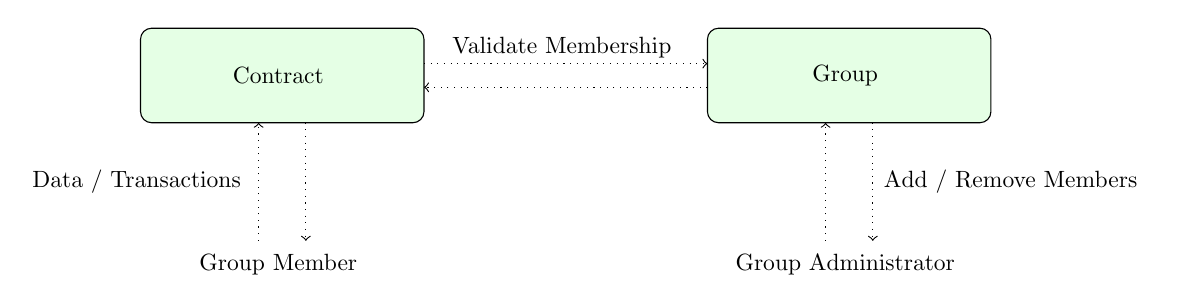
\begin{tikzpicture}[scale = 0.6, every node/.style={scale = 0.85}, every node/.append style={fill = white, rounded corners = 2pt, inner sep = 2pt, align = center}]

  \draw [rounded corners, fill=green!10] (-3, 1) rectangle (3, -1);
  \node [fill=green!10] at (0, 0) { Contract };

  \node at (-3, -2.25) { Data / Transactions };
  \draw [ -> , dotted] (-0.5, -3.5) -- (-0.5, -1);
  \draw [ -> , dotted] (0.5,  -1) -- (0.5,  -3.5);

  \node at (0, -4) { Group Member };

  \draw [rounded corners, fill=green!10] (9, 1) rectangle (15, -1);
  \node [fill=green!10] at (12, 0) { Group };

  \node at (15.5, -2.25) { Add / Remove Members };
  \draw [ -> , dotted] (11.5, -3.5) -- (11.5,    -1);
  \draw [ -> , dotted] (12.5,   -1) -- (12.5,  -3.5);

  \node at (12, -4) { Group Administrator };

  \node at (6, 0.6) { Validate Membership };
  \draw [ -> , dotted] (3,  0.25) -- (9,  0.25);
  \draw [ -> , dotted] (9, -0.25) -- (3, -0.25);

  \end{tikzpicture} \\
  \caption{
  	How a group interacts with an identity's data
  }
  \label{fig:archi_group_interactions}
\end{figure}


An identity claiming to be a member of a group will always interact with the storage contract it is trying to retrieve from or add data to. A group itself will never be able to directly affect or transact with a storage contract such that no malicious attacker would be able to pseudo-anonymously act as the group.

When the identity tries to access a path, their identity is cross-checked with the group they claim to be a member of. Should this group validate the identity as a member, and assuming the group has the necessary permissions that are required to action the identity's transaction, the transaction will be successful.

\paragraph{Group Key Sharing}

Whilst the process of writing data is similar to an individual (other than the membership validation above), the process of reading data differs hugely for groups.

If we were to extend the process of reading as an individual to a group, the result would be a process similar to that shown in figure \ref{fig:encryption_group_read_theoretical}.

\begin{figure}[H]
  \centering
  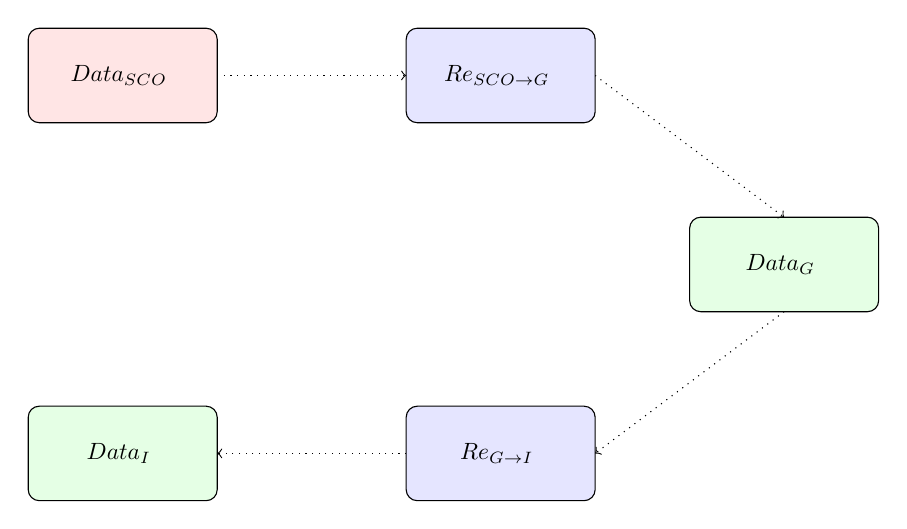
\begin{tikzpicture}[scale = 0.6, every node/.style={scale = 0.85}, every node/.append style={fill = white, rounded corners = 2pt, inner sep = 2pt, align = center}]

  \draw [rounded corners, fill=green!10] (-10, -7) rectangle (-6, -9);
  \node [fill=green!10] at (-8, -8) { $\text{Data}_{\text{I}}$ };

  \draw [ -> , dotted] (-2, -8) -- (-6, -8);

  \draw [rounded corners, fill=blue!10] (-2, -7) rectangle (2, -9);
  \node [fill=blue!10] at (0, -8) { $\text{Re}_{\text{G} \rightarrow \text{I}}$ };

  \draw [ -> , dotted] (6, -5) -- (2, -8);

  \draw [rounded corners, fill=green!10] (4, -3) rectangle (8, -5);
  \node [fill=green!10] at (6, -4) { $\text{Data}_{\text{G}}$ };

  \draw [ -> , dotted] (2, 0) -- (6, -3);

  \draw [rounded corners, fill=blue!10] (-2, 1) rectangle (2, -1);
  \node [fill=blue!10] at (0, 0) { $\text{Re}_{\text{SCO} \rightarrow \text{G}}$ };

  \draw [ -> , dotted] (-6, 0) -- (-2, 0);

  \draw [rounded corners, fill=red!10] (-6, 1) rectangle (-10, -1);
  \node [fill=red!10] at (-8, 0) { $\text{Data}_{\text{SCO}}$ };

  \end{tikzpicture} \\
  \caption{
  	Group Read Re-encryption (theoretical)
  }{
    The theoretical process of re-encrypting from a storage contract owner to a group, then re-encrypting again from the group to an individual (member of the group).
  }
  \label{fig:encryption_group_read_theoretical}
\end{figure}


Given the non-transitive nature of the proxy re-encryption scheme we are using, the process shown in figure \ref{fig:encryption_group_read_theoretical} doesn't allow end-to-end encryption. After the first stage of re-encryption, $\text{Data}_{G}$ represents a first-level encryption under the group $G$'s public key. Since the proxy re-encryption scheme being used only allows re-encryption from a second-level encryption to a first-level encryption (to eliminate transitivity), no further action is possible. Another process is required to facilitate group read.

Given only one re-encryption is possible, we look to the identity that the re-encryption is for. We ask ourselves whether the original (individual) scheme could work here, and indeed it could, although it comes with many flaws including:

\begin{itemize}
  \item 
  	\textbf{Non-optimal key storage} \\
    For every member of the group, a re-encryption key must be generated by the storage contract owner. The process of generating a re-encryption key for every member is $O(n)$, i.e. for a group with a membership of 50, 50 re-encryption keys need to be generated.
  % TODO: Need more here    
\end{itemize}

As an improvement to individual keys, let's take a look at the viability of the theoretical group read process. Assume that there is a group key pair, for which any data received by a member of the group from a storage contract is encrypted. Now all data is encrypted such that the group private key is required to decrypt it. The group private key is encrypted using the group public key such that it can only be decrypted by itself. The administrator of the group must therefore hold the re-encryption key from the group private key to their public key in order to read, and therefore administer, the group. When a member joins the group, the administrator creates a re-encryption key for them such that they are able to decrypt the group's private key when re-encrypted. However, when a member leaves the group, the reference to their re-encryption key is removed from the group contract.

In contrast to figure \ref{fig:encryption_group_read_theoretical}, the process of receiving data as a member of the group now follows a process similar to that shown in figure \ref{fig:encryption_group_read_practical}.

\begin{figure}[H]
  \centering
  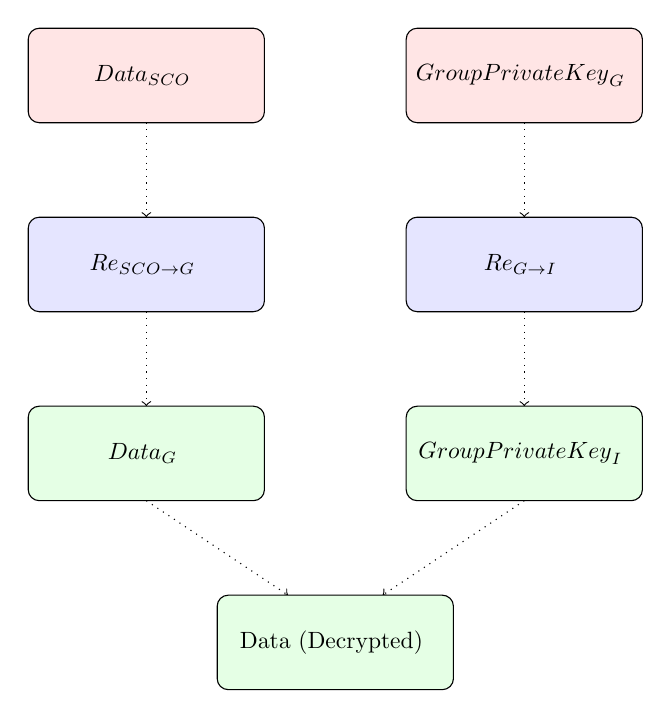
\begin{tikzpicture}[scale = 0.6, every node/.style={scale = 0.85}, every node/.append style={fill = white, rounded corners = 2pt, inner sep = 2pt, align = center}]

  % ------------------------------------------------------------------------

  \draw [rounded corners, fill=red!10] (-5.5, 1) rectangle (-10.5, -1);
  \node [fill=red!10] at (-8, 0) { $\text{Data}_{\text{SCO}}$ };

  \draw [ -> , dotted] (-8, -1) -- (-8, -3);

  \draw [rounded corners, fill=blue!10] (-5.5, -3) rectangle (-10.5, -5);
  \node [fill=blue!10] at (-8, -4) { $\text{Re}_{\text{SCO} \rightarrow \text{G}}$ };

  \draw [ -> , dotted] (-8, -5) -- (-8, -7);

  \draw [rounded corners, fill=green!10] (-5.5, -7) rectangle (-10.5, -9);
  \node [fill=green!10] at (-8, -8) { $\text{Data}_{\text{G}}$ };

  % ------------------------------------------------------------------------

  \draw [rounded corners, fill=red!10] (-2.5, 1) rectangle (2.5, -1);
  \node [fill=red!10] at (0, 0) { $\text{Group Private Key}_{\text{G}}$ };

  \draw [ -> , dotted] (0, -1) -- (0, -3);

  \draw [rounded corners, fill=blue!10] (-2.5, -3) rectangle (2.5, -5);
  \node [fill=blue!10] at (0, -4) { $\text{Re}_{\text{G} \rightarrow \text{I}}$ };

  \draw [ -> , dotted] (0, -5) -- (0, -7);

  \draw [rounded corners, fill=green!10] (-2.5, -7) rectangle (2.5, -9);
  \node [fill=green!10] at (0, -8) { $\text{Group Private Key}_{\text{I}}$ };

  % ------------------------------------------------------------------------

  \draw [ -> , dotted] (-8, -9) -- (-5, -11);
  \draw [ -> , dotted] (0, -9) -- (-3, -11);

  \draw [rounded corners, fill=green!10] (-6.5, -11) rectangle (-1.5, -13);
  \node [fill=green!10] at (-4, -12) { Data (Decrypted) };

  % ------------------------------------------------------------------------

  \end{tikzpicture} \\
  \caption{
  	Group Read Re-encryption (practical)
  }{
    The practical process of re-encrypting from a storage contract owner to a group, re-encrypting a group key from the group to an individual (member of the group), and combining the two to provide the decrypted data.
  }
  \label{fig:encryption_group_read_practical}
\end{figure}

